\section{電流パルスを用いたパルス加熱・急冷実験の手法}
%相転移の実験は光学クライオスタット中のヘリウムガス
本章では電流パルスを用いたαスズからβスズへの変換と共存状態生成に関する実験手法について説明する。

\subsection{Sn-Ge合金への端子付け}

\subsubsection{端子づけに用いた道具}
\begin{itemize}
\item 乾いた毛筆($250\mu m$程度)
\item 乾いた毛筆($500\mu m$程度)
\item 毛筆(銀ペースト用)
\item 毛筆(グリース用)\\
(*毛筆は用途によって印をつけておく(たとえば黒の塗りつぶし:銀ペースト;縞模様:細い)。毛は1mm程度の長さが良いと思う。長すぎると金線やサンプルを飛ばしてしまう。)
\item 銀ペーストを練るようじ
\item ピンセット
\item キムワイプ
\end{itemize}

材料・そのほかに便利な道具:
\begin{itemize}
\item 金線(太さ250um)
\item 銀ペースト
\item 光学顕微鏡
\item 金線を切るためのハサミ
\item 金線を置いておくゴムマット
\item 銀ペーストを練るスライドガラス
\item サンプル近くに置く銀ペーストのパレット
\item サンプルとパレットを乗せるスライドガラス
\item ユニバーサル基板(ピッチ2.5mm)
\item 両面テープ
\end{itemize}

毛筆の作り方:
\begin{enumerate}
\item 二液式接着剤を混ぜてつまようじの先に薄くつける
\item 一本の毛(腕毛、すね毛、まつげ、髪の毛など)を、接着剤に先を出して埋め込む
\item  接着剤が乾いたら、毛の長さをはさみで調整する
 \end{enumerate}

\subsubsection{作業を始める前に} 
\begin{itemize}
\item 前日はよく寝る
\item 机の上を整理整頓
\item 空調のスイッチを切る(作業終了後は再度スイッチを入れる)
\item 左右の接眼レンズの間隔とピントを調整する
\item 椅子の高さを調整
\end{itemize}
 
\subsubsection{四端子付けの手順} 
1. 準備
\begin{itemize}
\item ユニバーサル基板を適当な大きさにカットする
\item スライドガラスに両面テープでユニバーサル基板を貼り付ける。このとき銀ペーストを伸ばすパレットを横に作る。
\item 金線を必要なぶん切っておく(まっすぐで長さのそろった、汚れていないものが扱いやすい)
\item 銀ペーストをよく練って、サンプル横のパレットに適量のせる
\end{itemize}
 
2. サンプルの仮留め
\begin{itemize}
\item 基板にグリースを毛筆で少量つける。毛筆で伸ばす必要はない
\item 毛筆の先にグリースを微量つけてサンプルを持ち上げ、ユニバーサル基板につけたグリースの上に置く
\item サンプルを上から軽く押して、密着させる
\end{itemize}
 
3. 電流端子2本の取り付け
\begin{itemize}
\item まず金線一本をピンセットと毛筆で移動する。一方の端がサンプルの近くで、もう一方がユニバーサル基板の銅箔の近くにくるようにする
\item 金線と銅箔を銀ペーストでくっつける。銀ペーストが固まる前に、サンプル側の端がサンプルに触れるように微調整する
\item もう一本の金線に関しても同様に、銅箔と金線を銀ペーストでくっつけて固まるまで待つ
\item 銅箔側の銀ペーストが固まったら、サンプルと金線を銀ペーストでつなぐ。流れる電流がなるべく一様な密度になるように、横に広く接続することを意識する
 \end{itemize}
 
4. サンプルの持ち上げ
\begin{itemize}
\item サンプルと金線の間の銀ペーストが固まったら、金線と基板の間に毛筆を入れてサンプルを持ち上げる
 \end{itemize}
 
5. 電圧端子2本の取り付け
\begin{itemize}
\item 電流端子と同様に接続する。ただし、銀ペーストがサンプルに触れる面積が小さくなるように心がける。また測定中の低温でユニバーサール基板や金線が収縮して、サンプルと接合点に強い応力がかかるのを防ぐため、金線をユニバーサル基板の銅箔につけて固めた後少し曲げるとよいと思う。
 \end{itemize}
 
6. そのほか端末の取り付け
\begin{itemize}
\item PPMSのための端末をつくる
\end{itemize}

7. 最後に
\begin{itemize}
\item 記録のため写真をとっておく
\item 4端子間の抵抗を測定して3オーム程度であることを確認する
\end{itemize}
 

\subsubsection{作業が終わったら} 
\begin{itemize}
\item 空調の電源をオンにする
\item 顕微鏡の照明をオフにする
\item 机の上の片付け
\item サンプルをデシケータに入れる
\end{itemize}
 
\subsubsection{作業のコツ} 
ピンセット
\begin{itemize}
\item 汚れたらキムワイプで拭いて先を綺麗に保つ
\item 金線はつよく掴まない、できるだけ平行につまむ
\item 先を保護するために、金線はゴムマットの上でつまむ
\end{itemize}
 
毛筆の使い方
\begin{itemize}
\item 銀ペーストを塗ったあとは毛を溶媒で洗って、キムワイプで拭く
\item つまようじを人差し指と中指で持つと疲れない
\item 小指の付け根を台につけて、左手を添えると震えにくい
\end{itemize}

銀ペーストの取り扱い
\begin{itemize}
\item 溶媒(コハク酸ジエチル)の液溜まりと固い銀ペーストの塊はスライドガラス上に離しておく。銀ペーストは少しずつ溶かして混ぜる。液溜まりでは銀ペーストを塗ったあとの毛筆を洗う。
\item パレットの銀ペーストは乾きやすいので、定期的に溶媒を足して練り直す
\item サンプルと金線を接続するときは、まず薄いペーストの表面張力でくっつける。乾くのを待って、濃いペーストで形を整える。はみ出した時は細く切った(2*20mm)キムワイプの先をちぎってねじったものに溶媒を含ませて拭く
\end{itemize}

その他
\begin{itemize}
\item 顕微鏡の倍率:高倍率で固定して、毛筆やピンセットはなるべく動かさない。スライドガラスとサンプルを動かすようにする
\item 休憩:一時間半に少なくとも一度休憩するのが望ましい
\end{itemize}

四端子測定が上手くいかない時
\begin{itemize}
\item 光学顕微鏡像の画像をとって、測定前と比べてみる
\item 各端子間の抵抗を測ってみる
\item 毛筆で端子を触ってみる
\end{itemize}

\subsubsection{電流パルス実験の際の技術的な工夫} 
スズの相転移には大きな体積変化が伴うため、電流パルスにより試料の温度を上げて相転移を起こし、端子がくっついた状態を維持するためにはいくつかの技術的な工夫が欠かせない。本節ではその技術的な工夫とその手法に至るまでの失敗例を説明する。

まずファーストトライアルにおいて、筆者は直径$\rm 25 \mu m$の金線を電圧・電流端子として銀ペーストで試料に接続した。その試料を25Kに保持し電流パルスを印加したところ、試料が相転移温度に達するまえに直径$\rm 25 \mu m$の金線からなる電流端子が焼き切れた。そのときの電流は1.3A程度だった。したがって電流端子に繋ぐ金線は$\rm 25 \mu m$より太いものに取り替える必要がある。また数A程度の電流を流すと試料付近以外でも発熱し断線のリスクがあるため、あえて試料付近に高抵抗(ヒーター)の領域を作って発熱効率を高める必要がある。

そこで、次に筆者はカーボンペーストで直径$\rm 50 \mu m$の金線を接続することで、効果的に試料を加熱しながら、かつ金線が焼き切れないような構成を目指した。しかしこの構成では試料が相転移温度に達するまえに、カーボンペーストによる接続部が過熱で壊れてしまった。この結果はカーボンペーストは銀ペーストに比べ抵抗が高い反面、機械強度が弱いことに起因する。またカーボンペーストを用いた電気的な接続では、カーボンペーストの高い抵抗率に起因して発熱部分が試料と金線の間に集中してしまう。

筆者は試行錯誤の結果、図\ref{fig:schematics_sample}のような端子の接続法を見出した。付録\ref{sec:4terminal}に示すように、カーボンペーストは発熱に十分に高い抵抗が実現できる一方で機械的な強度が低く、銀ペーストは強度が高い一方で抵抗が小さい。これらを効果的に組み合わせることで、筆者は機械的強度と高抵抗を確保できると筆者は考えた。そこでカーボンペーストで金線をコーティングした後、銀ペーストで覆い試料にしっかりと接続した。この構成では低抵抗率の銀ペーストが挟まっているので試料と金線の間に電流経路が集中せず、比較的一様な発熱が可能となったと考える。また電流端子につなぐ金線は1A程度以下の電流で焼き切れないように直径$\rm 50 \mu m$のものとした。一方電圧端子をつなぐ線には大電流が流れないため、試料に応力をかけないよう柔らかく、熱伝導の高すぎないものとしたかった。そこで直径$\rm 25 \mu m$の金線とした。
\begin{figure}[!h]
    \begin{center}
   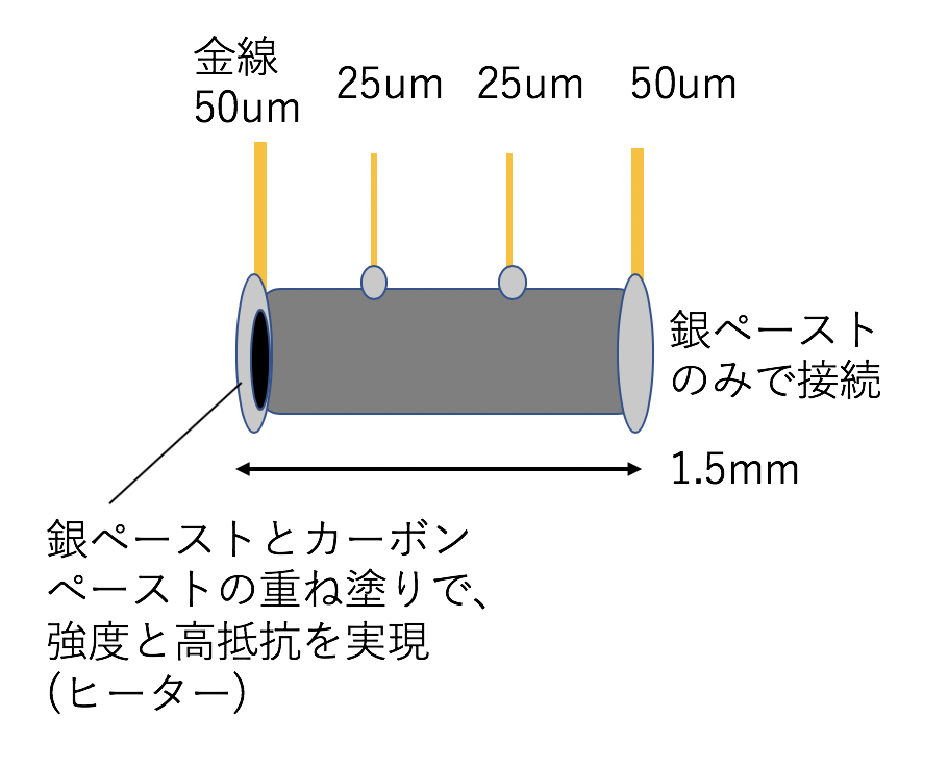
\includegraphics[width=0.4\hsize]{experiment/schematics_sample.eps}
  \end{center}
  \caption{}
  \label{fig:schematics_sample}
\end{figure}

\subsection{α相からβ相への変換}
まずパルス印加の前に抵抗の温度依存性も測定した。抵抗の温度依存性を測定するときの電気回路の模式図を図\ref{fig:schematics_lockin}に示す。ロックインアンプ(Stanford Research SR830)から出力した105Hzの交流電圧は、光学クライオスタット中の試料とロード抵抗の直列接続に印加される。回路に流れる電流は$\rm 150\Omega$のロード抵抗の電圧降下をマルチメータ(Keithley 2001)で読み取り算出した。試料の電圧端子間の電圧効果はトランス増幅器(Stanford Research SR554)で100倍に増幅したあと、ロックインアンプの入力端子に入力した。回路に流す電流値は、25Kの試料にパルス電流を印加したとき温度上昇しなかった値より十分小さくとった。また試料の複素インピーダンスの虚部(位相進み/遅れ)成分は実部の1/100程度以下だったので無視して、実部のみを抵抗とした。
\begin{figure}[!h]
     \begin{center}
   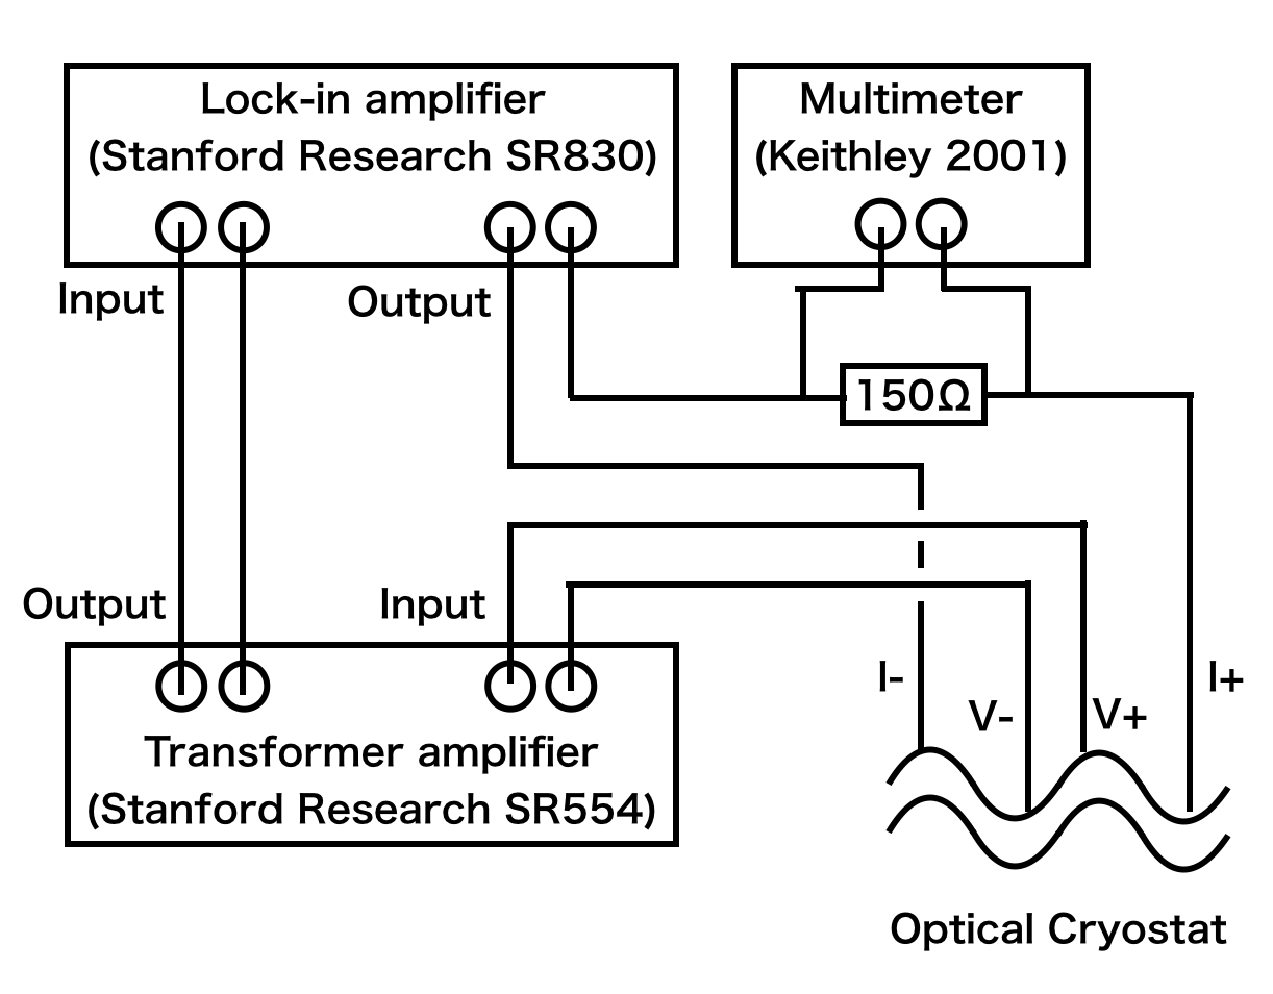
\includegraphics[width=0.5\hsize]{experiment/schematics_lockin.eps}
  \end{center}
  \caption{}
  \label{fig:schematics_lockin}
\end{figure}


抵抗の温度依存性を測定した後αスズからβスズに相転移を起こすことを目的として、25Kに保った試料に孤立した電流パルスを3秒印加してジュール発熱により加熱した。スズ相転移前後で抵抗が大きく異なるため、相転移の確認はパルス印加中の抵抗変化を測定することで行った。その際用いた電気回路の模式図を図\ref{fig:schematics_pulse}に示す。ソースメータ(Keithley 2400)から出力されたパルス電圧は、パワーアンプ(NF Corp. 4502)で100倍に増幅されたあと、光学クライオスタット中の試料とロード抵抗の直列接続に印加される。回路に流れる電流の時間変化は、$\rm 5.4\Omega$のロード抵抗の電圧降下をデータロガー(MC DT8824)で読み取り計算した(Ch2)。また試料の電圧降下もデータロガー(MC DT8824)で読み取り計算した(Ch1)
\begin{figure}[!h]
 \begin{minipage}{0.5\hsize}
    \begin{center}
   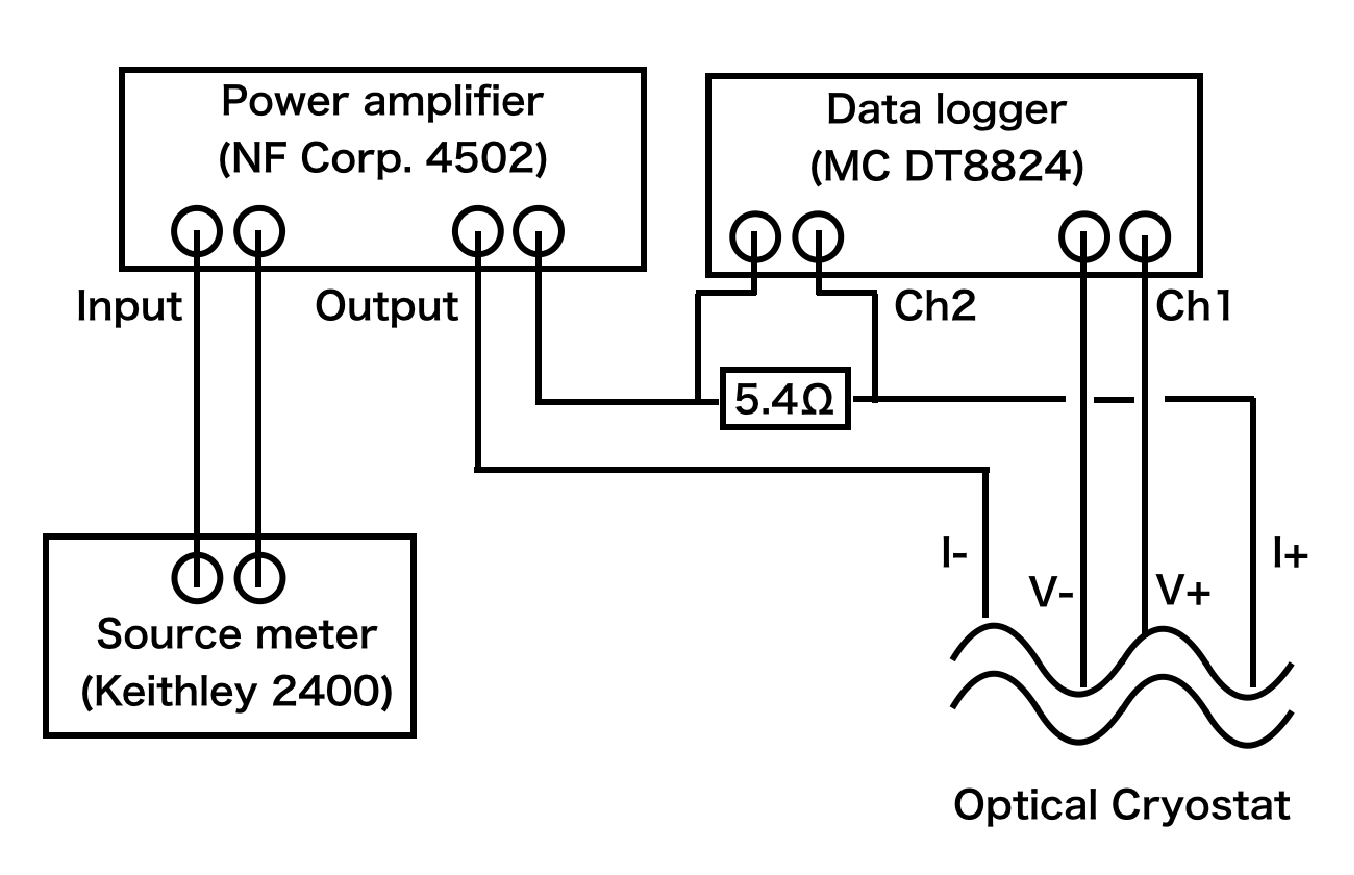
\includegraphics[width=\hsize]{experiment/schematics_pulse.eps}
  \end{center}
  \caption{}
  \label{fig:schematics_pulse}
   \end{minipage}
    \begin{minipage}{0.4\hsize}
       \begin{center}
   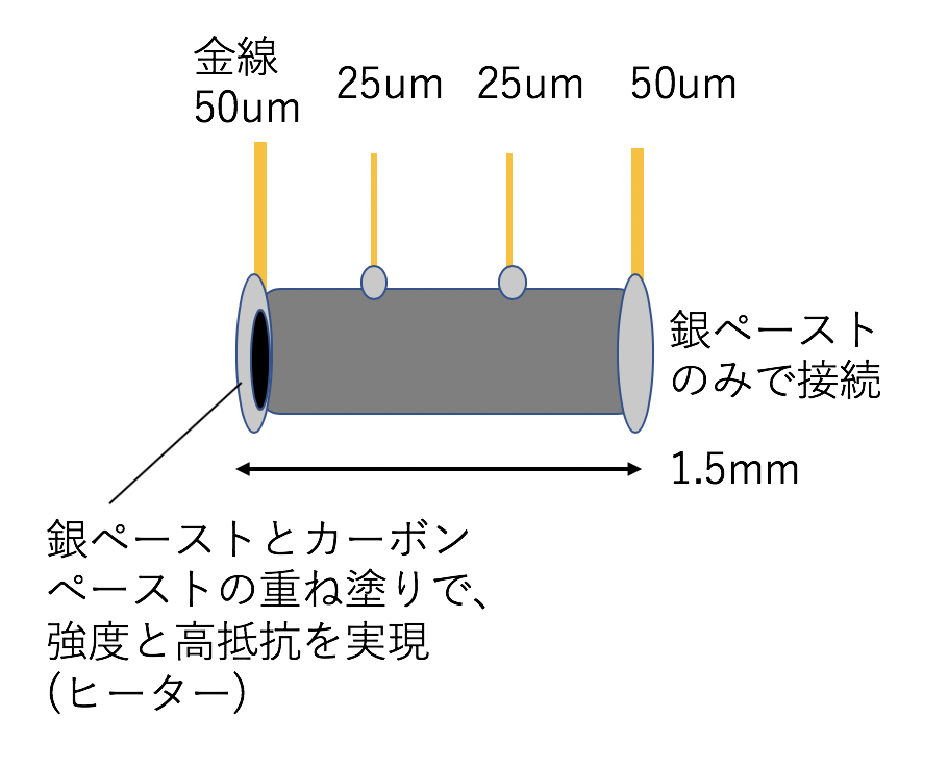
\includegraphics[width=\hsize]{experiment/schematics_sample.eps}
  \end{center}
  \caption{}
  \label{fig:schematics_sample}
    \end{minipage}
  \end{figure}
  
効果的に試料を加熱するために筆者は図\ref{fig:schematics_sample}のような端子の接続法を用いた。\ref{sec:4terminal}に述べるように、カーボンペーストは発熱に十分に高い抵抗が実現できる一方で機械的な強度が低く、銀ペーストは強度が高い一方で抵抗が小さい。これらを効果的に組み合わせることで、筆者は機械的強度と高抵抗を確保できると筆者は考えた。そこでカーボンペーストで金線をコーティングした後、銀ペーストで覆い試料にしっかりと接続した。この構成では低抵抗率の銀ペーストが挟まっているので試料と金線の間に電流経路が集中せず、比較的一様な発熱が可能となったと考える。また電流端子につなぐ金線は1A程度以下の電流で焼き切れないように直径$\rm 50 \mu m$のものとした。一方、電圧端子をつなぐ線には大電流が流れないため、柔らかく熱伝導の高すぎないものとしたかった。そこで直径$\rm 25 \mu m$の金線とした。

電流パルスを印加した後にふたたび試料抵抗の温度依存性を測定した。パルス印加前と同様に図\ref{fig:schematics_lockin}の電気回路を用いた。

\subsection{αスズとβスズの共存状態の生成}
次に電流パルスを印加してαスズを部分的にβスズに変換し、αスズとβスズの共存状態を生成することを目指した。序論で述べた通りαスズとβスズはともに温度200K以下と室温で安定である。室温でもパルス印加で相転移が示せれば極めて有用と筆者は考える。さらに低温での実験に比べ冷媒を必要とせず、簡便で実験の自由度も大きい。そこで本実験では室温に保った試料に電流パルスを印加した。

本実験に用いた電気回路は前節のパルス印加実験と同様である。ただし図\ref{fig:schematics_sample2}のように電流端子の片側のみにカーボンペーストを用いた点が異なる。主に片側のみから発熱させることで意図的に試料内の温度勾配を作り出し、部分的な書き込みを制御した。カーボンペーストを用いて接続する方法は前節と同様である(\ref{sec:4terminal})。
\begin{figure}[!h]
 \begin{minipage}{0.4\hsize}
    \begin{center}
   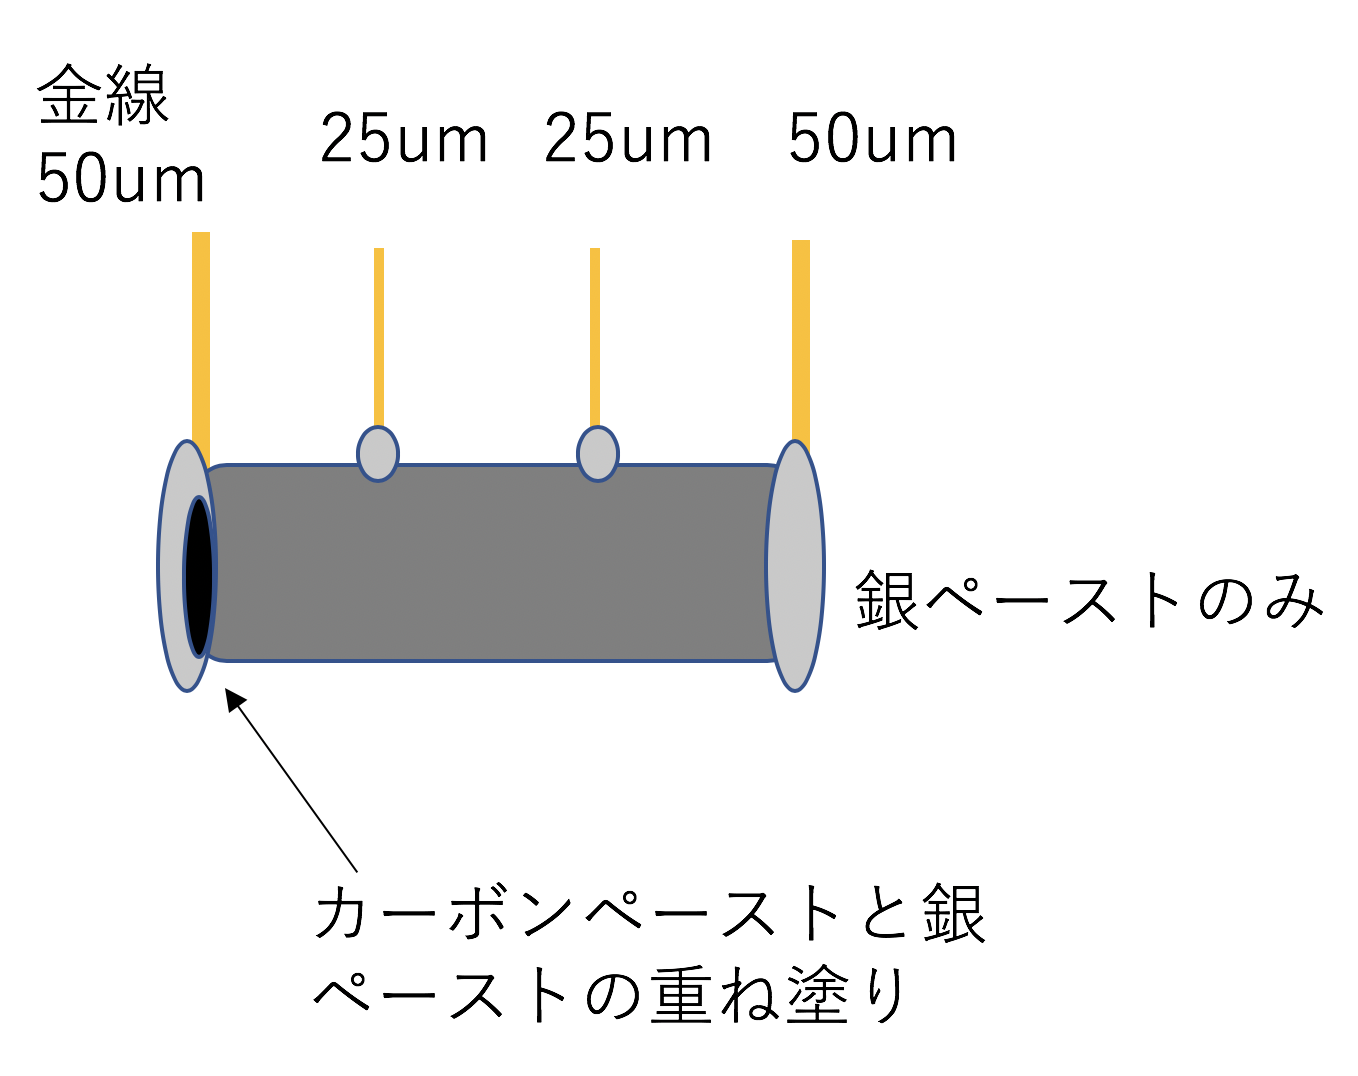
\includegraphics[width=\hsize]{experiment/schematics_sample2.eps}
  \end{center}
  \caption{}
  \label{fig:schematics_sample2}
   \end{minipage}
 \begin{minipage}{0.35\hsize}
    \begin{center}
   \includegraphics[width=\hsize]{experiment/microscope.eps}
  \end{center}
  \caption{}
  \label{fig:microscope}
   \end{minipage}
\end{figure}

また顕微光学系を構成し、パルス印加中の試料を光学的に観察した。図\ref{fig:microscope}に顕微光学系の模式図を示す。光源から照明を入射する際に、顕微光学系の光軸から外した配置とすることで迷光を抑え、コントラストの大きな動画・画像を撮影した。


本実験ではパルス幅1秒、インターバル1秒のパルス列を試料に印加した。

%\subsection{電流パルスを用いたβ相からα相への変換}

\clearpage

%\ref{sec:4terminal}